% This file was created by tikzplotlib v0.9.1.
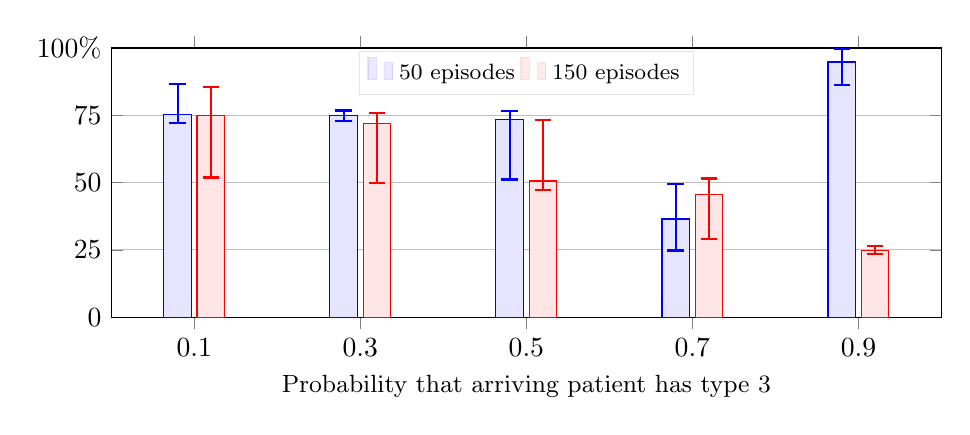
\begin{tikzpicture}

% \definecolor{color0}{rgb}{0.12156862745098,0.466666666666667,0.705882352941177}
% \definecolor{color1}{rgb}{1,0.498039215686275,0.0549019607843137}

\begin{axis}[
    % % /pgf/number format/.cd,
    %     % use comma,
    % height = 7cm,
    % width = 8.5cm,
    % ymajorgrids,
    % % ylabel={The mighty Force in \si{\newton}},
    % % xlabel={A strong Opponent},
    % ymin = 0,
    % ymax= 1.75,
    % ybar=0pt,
    % bar width=12pt,
    % enlarge x limits = 0.3,
    % nodes near coords,
    % % point meta=explicit symbolic,
    % % scatter/position=absolute,
    % % every node near coord/.style={
    %     % at={(\pgfkeysvalueof{/data point/x},1.8)},
    %     % anchor=south,
    % % },
    % bar shift=0pt,
    % % xtick={0,1,2},
    % % xticklabels={metal,wood,paper},
    % % x tick label style={rotate=45,anchor=east},
    ybar,
    % % enlargelimits = 0.15,
    width = \columnwidth,
    % % heigth = \axisdefaultheight,
    height = 5cm,
    % legend cell align={left},
    % legend style={
    %     font=\footnotesize,
    %     fill opacity=0.8,
    %     draw opacity=1,
    %     text opacity=1,
    %     at={(0.03,0.07)},
    %     anchor=south west,
    %     draw=white!80!black
    % },
    legend style={
        font=\footnotesize,
        fill opacity=0.8,
        draw opacity=0.1,
        text opacity=1,
        at={(0.5,0.99)},
        anchor=north,
        legend columns=-1
    },
    % tick align=outside,
    % tick pos=left,
    x grid style={white!69.0196078431373!black},
    xlabel={\small Probability that arriving patient has type 3 },
    xmin=0,
    xmax=1,
    % xtick style={color=black},
    % % xtick={0, 0.2, 0.4, 0.6, 0.8, 1},
    % % xticklabels={0,0.2,0.4,0.6,0.8,1},
    xtick={0.1, 0.3, 0.5, 0.7, 0.9},
    xticklabels={0.1, 0.3, 0.5, 0.7, 0.9},
    % % symbolic x coords = {0.1, 0.3, 0.5, 0.7, 0.9},
    % y grid style={white!69.0196078431373!black},
    ymin=0,
    ymax=100,
    ytick={0, 25, 50, 75, 100},
    yticklabels={0, 25, 50, 75, 100\%},
    % ytick style={color=black},
    error bars/y dir=both,
    error bars/y explicit=true,
    error bars/error bar style={thick},
    error bars/error mark options={
          rotate=90,
          % red,
          mark size=3pt,
          % line width=1pt
          thick,
    },
    ymajorgrids,
]

\addplot [
    fill=blue!10!white,
    draw = blue,
    error bars/error mark options/.append={blue}
] table [
    x=x,
    y=y,
    y error minus=y_lower,
    y error plus=y_upper
] {
x      y       y_lower  y_upper
0.1    75.4     3.2    11.2
0.3    75.      2.      1.8
0.5    73.4    22.2     3.2
0.7    36.5    11.7    13.1
0.9    94.8     8.64    4.8
};
\addlegendentry{50 episodes}

\addplot [
    fill=red!10!white,
    draw = red,
    % error bars/.cd,
    error bars/error mark options/.append={red}
] table [
    x=x,
    y=y,
    y error minus=y_lower,
    y error plus=y_upper,
] {
x      y       y_lower  y_upper
0.1  74.9    22.98    10.5
0.3  72.     22.04     3.84
0.5  50.6     3.48    22.8
0.7  45.6    16.64     5.92
0.9  24.9     1.54     1.54
};
\addlegendentry{150 episodes}

\end{axis}

\end{tikzpicture}



%% 50 episodes
% Error bars
% \path [draw=color0]
% (axis cs:0.1,72.2)
% --(axis cs:0.1,86.6);
% \path [draw=color0]
% (axis cs:0.3,73)
% --(axis cs:0.3,76.8);
% \path [draw=color0]
% (axis cs:0.5,51.2)
% --(axis cs:0.5,76.6);

% \path [draw=color0]
% (axis cs:0.7,24.8)
% --(axis cs:0.7,49.6);
% \path [draw=color0]
% (axis cs:0.9,86.16)
% --(axis cs:0.9,99.6);

% % Tick marks error bars
% \addplot [semithick, color0, mark=-, mark size=2, mark options={solid}, only marks]
% table {%
% 0.1 72.2
% 0.3 73
% 0.5 51.2
% 0.7 24.8
% 0.9 86.16
% };
% \addplot [semithick, color0, mark=-, mark size=2, mark options={solid}, only marks]
% table {%
% 0.1 86.6
% 0.3 76.8
% 0.5 76.6
% 0.7 49.6
% 0.9 99.6
% };

% % Line
% \addplot [semithick, color0]
% table {%
% 0.1 75.4
% 0.3 75
% 0.5 73.4
% 0.7 36.5
% 0.9 94.8
% };
% \addlegendentry{50 episodes}

% %% 150 episodes
% % % Error bars
% % \path [draw=color1]
% % (axis cs:0.105,51.92)
% % --(axis cs:0.105,85.4);
% % \path [draw=color1]
% % (axis cs:0.305,49.96)
% % --(axis cs:0.305,75.84);
% % \path [draw=color1]
% % (axis cs:0.505,47.12)
% % --(axis cs:0.505,73.4);
% % \path [draw=color1]
% % (axis cs:0.705,28.96)
% % --(axis cs:0.705,51.52);
% % \path [draw=color1]
% % (axis cs:0.905,23.36)
% % --(axis cs:0.905,26.44);

% % % Tick marks error bars
% % \addplot [semithick, color1, mark=-, mark size=2, mark options={solid}, only marks]
% % table {%
% % 0.105 51.92
% % 0.305 49.96
% % 0.505 47.12
% % 0.705 28.96
% % 0.905 23.36
% % };
% % \addplot [semithick, color1, mark=-, mark size=2, mark options={solid}, only marks]
% % table {%
% % 0.105 85.4
% % 0.305 75.84
% % 0.505 73.4
% % 0.705 51.52
% % 0.905 26.44
% % };

% % % Line
% % \addplot [semithick, color1]
% % table {%
% % 0.105 74.9
% % 0.305 72
% % 0.505 50.6
% % 0.705 45.6
% % 0.905 24.9
% % };

% % \addlegendentry{150 episodes}


% \addplot+ [
%     error bars/.cd,
%     y dir=both, y explicit,
% ] coordinates {
% (0.1, 75.4) -= (0,  3.2) += (0, 11.2)
% (0.3, 75. ) -= (0,  2. ) += (0,  1.8)
% (0.5, 73.4) -= (0, 22.2) += (0,  3.2)
% (0.7, 36.5) -= (0, 11.7) += (0, 13.1)
% (0.9, 94.8) -= (0, 8.64) += (0,  4.8)
% };

% Data 50 episodes (median, lower, upper)
% (array([]), array([[ 3.2 ,  2.  , 22.2 , 11.7 ,  8.64], []]))

% Data 150 episodes
% (array([74.9, 72. , 50.6, 45.6, 24.9]), array([[22.98, 22.04,  3.48, 16.64,  1.54], [10.5 ,  3.84, 22.8 ,  5.92,  1.54]]))


% \path [draw=color1]
% (axis cs:0.1,21)
% --(axis cs:0.1,25.64);
% 
% \path [draw=color1]
% (axis cs:0.3,23.2)
% --(axis cs:0.3,26.8);
% 
% \path [draw=color1]
% (axis cs:0.5,23.6)
% --(axis cs:0.5,26.8);
% 
% \path [draw=color1]
% (axis cs:0.7,23.4)
% --(axis cs:0.7,26.6);
% 
% \path [draw=color1]
% (axis cs:0.9,23.2)
% --(axis cs:0.9,26.4);
% \addplot [semithick, color1, mark=-, mark size=2, mark options={solid}, only marks]
% table {%
% 0.1 21
% 0.3 23.2
% 0.5 23.6
% 0.7 23.4
% 0.9 23.2
% };
% \addplot [semithick, color1, mark=-, mark size=2, mark options={solid}, only marks]
% table {%
% 0.1 25.64
% 0.3 26.8
% 0.5 26.8
% 0.7 26.6
% 0.9 26.4
% };

% \addplot [semithick, color1]
% table {%
% 0.1 23.6
% 0.3 25
% 0.5 25.2
% 0.7 24.8
% 0.9 24.6
% };

